% standalone permite compilar por separado
\documentclass[10pt,margin=8pt]{standalone}
\usepackage[utf8]{inputenc}
\usepackage{tikz}
\usetikzlibrary{decorations.text} %Para soportar la decoiración con textos
\begin{document}
	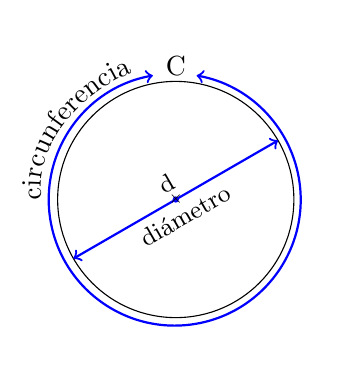
\begin{tikzpicture}
		\draw(0,0) circle[radius=1.5cm];
		\fill[blue] circle[radius=0.4mm]node[below,rotate=30,black]{\small diámetro};
		\draw[<->, thick, blue,rotate=30] (-1.5,0) to (1.5,0) node[pos=.6,above, black] {\small d};
		\node at (0,0){\tiny $\times$};
		\draw[<->, thick, blue, rotate=80](1.5,.56)arc(20:360:1.6);
		\node at (0,1.7) {C};
		\path[decorate, decoration={text along path, text={circunferencia}}][out=100](-1.7,0) to [in=139](.5,1.5);
	\end{tikzpicture}
	
	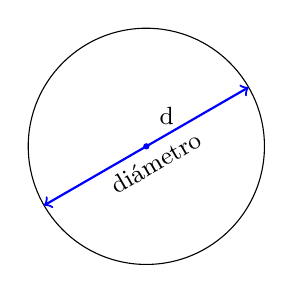
\begin{tikzpicture}
		\draw(0,0) circle[radius=1.5cm];
		\fill[blue] circle[radius=0.4mm]node[below,rotate=30,black]{\small diámetro};
		\draw[<->, thick, blue,rotate=30] (-1.5,0) -- (1.5,0) node[pos=.6,above, black] {\small d};
	\end{tikzpicture}
	
	
\end{document}	